
%%%%%%%%%%%%%%%%%%%%%%%%%%%%%%%%%%%%%%%%%%%%%%%%%%%%%%%%%%%%%%%%%%%%%%%%%%%%%%%%
%2345678901234567890123456789012345678901234567890123456789012345678901234567890
%        1         2         3         4         5         6         7         8

%\documentclass[letterpaper, 10 pt, conference]{ieeeconf}  % Comment this line out if you need a4paper

\documentclass[a4paper, 10pt, conference]{ieeeconf}      % Use this line for a4 paper
\usepackage[T1]{fontenc}
\IEEEoverridecommandlockouts                              % This command is only needed if
                                                          % you want to use the \thanks command

\overrideIEEEmargins                                      % Needed to meet printer requirements.

% See the \addtolength command later in the file to balance the column lengths
% on the last page of the document

% The following packages can be found on http:\\www.ctan.org
%\usepackage{graphics} % for pdf, bitmapped graphics files
%\usepackage{epsfig} % for postscript graphics files
%\usepackage{mathptmx} % assumes new font selection scheme installed
%\usepackage{times} % assumes new font selection scheme installed
\usepackage{amsmath} % assumes amsmath package installed
%\usepackage{amssymb}  % assumes amsmath package installed
\usepackage{algorithm}% http://ctan.org/pkg/algorithm
\usepackage{algpseudocode}% http://ctan.org/pkg/algorithmicx
\usepackage{graphicx}
\usepackage{moreverb}

\title{\LARGE \bf Project Report \\ EDAN70 Project in Computer Science \\ Intelligent Systems \\ Classifying Laser Range Data "Images" \\ Supervisor: Elin Anna Topp}
\date{\today}
\author{Fredrik Paulsson \\ dat11fp1@student.lu.se \and Shan Senanayake \\ dat11sse@student.lu.se}


\begin{document}
\maketitle
\thispagestyle{empty}
\pagestyle{empty}


%%%%%%%%%%%%%%%%%%%%%%%%%%%%%%%%%%%%%%%%%%%%%%%%%%%%%%%%%%%%%%%%%%%%%%%%%%%%%%%%
%\begin{abstract}

%This electronic document is a �live� template. The various components of your paper [title, text, heads, etc.] are already defined on the style sheet, as illustrated by the portions given in this document.

%\end{abstract}


%%%%%%%%%%%%%%%%%%%%%%%%%%%%%%%%%%%%%%%%%%%%%%%%%%%%%%%%%%%%%%%%%%%%%%%%%%%%%%%%
\section{INTRODUCTION}

In this project we are to develop a classifier that takes as input laser range data and output a classification of the data. The classification may be \emph{door}, \emph{wall} and similar objects.

The goal is to implement this as a ROS node in C++ that can run online on a robot.

The project consists of several parts. The first part is to develop a parser for the laser range data that will put the data in some kind of a data structure as well as transforming the represenation into a form that is easier to work with.

The second part is to develop and implement an algorithm that has the abillity to classify the laser range data. This algorithm is supposed to operate within the data structures that our parser has created.

The third part is to port the classifier into a ROS node and test it in an online environment running on the robot. During development we will use laser range data that has been gathered in the past.

This report will serve as documentation of our project.

\section{Machine Learning}
We are both very interested in machine learning and has therefore decided to develop our classifier within the machine learning area of artificial intelligence.

The idea that we have is to combine both supervised and unsupervised learning for use in order to classify laser range data. We will start of by manually classifying some data and put it into a database. When the classifier is used it will browse the database and find out which laser range data in the database that matches best with the data to be classified. It will then give the new data the same classification as the data that matched best.

There should be a threshold on how much the best match in the database must match the new data. If this threshold is crossed the classifier will either be unable to give a classification, give an "unknown" classification or simply prompt a warning that this classification may be wrong.

\section{PARSER}
The offline data of measurements that we have used to test our classifier and based the supervised learning part on was given to us in a specific format. All measurements gathered in one run of the robot's laser range scanner is put into one single file called \emph{scans.dat}. Each single measurement is placed on its own line. Measurements were gathered with a frequency of 4-5 Hz according to our supervisor.

Each of these measurements had a specific format and each measurements starts with a header of 15 values and then a value for each point in the measurement. The laser range scanner works by emitting a certain number of laser beams which will be reflected in obejcts in the field of view of the scanner. The scanner will then calculate the distance to each reflection point resulting in a number of distances. In each measurements the number of points and the angle between the points are given. Effectively each point's coordinates is given in polar form.

Each measurement looks like the following:

\begin{verbatim}
<unknown> <unknown> <number_of_points>
<timestamp_seconds> <timestamp_microseconds>
<unknown> <unknown> <unknown> <unknown>
<unknown> <unknown> <angle_between_points>
<unknown> <unknown> <unknown>
<distance_in_meters>^<number_of_points>
\end{verbatim}

As can be seen there are a lot of unknown values that we do not know and that our supervisor could not explain to us. However, these values are not needed by us in this project. The most important values are the number of points, the angle between the points and for each point the distance to the point.

Directly parsing the above format of each mesurement yields polar coordinates. Polar coordinates are very hard to work with as they are not easily visualized or easily worked with. This made us constructing a transformation of these polar coordinates into our own cartesian coordinate system.

Our coordinate system is based on some basic principles. The robot is positioned at origin and is the front of the robot is along the y-axis. This is basically the standard way to transform between polar and cartesian coordinates. The only special this is that the angle for the polar coordinates is expressed from the starting point. However, the starting point may be located at different angles from the x-axis depending on the specific type of laser range scanner. Different scanners may have a different number of points, different angle between the points and differently sized fields of view. With field of view we mean the entire angle that the scanner scans. In order to manage this problem we chose to express the angle from the y-axis instead and thus replace the use of sinus and cosinus with each other in the standard transform and also to manage the sign of each coordinate.

Now that we had coordinates in a much more manageable represenation we could visualize the data for ourself and we could use standard mathematical formulas in order to work with each measurement. As we needed to manually classify measurements in order to feed these to the classifier as a starting ground it was vital that we could easily plot the measurements. This was easily done in Matlab or Octave when we had our cartesian coordinates. Figures \ref{human}, \ref{doorhalf}, \ref{doorfull} and \ref{chair} shows som example plots.


\begin{figure}
\centering
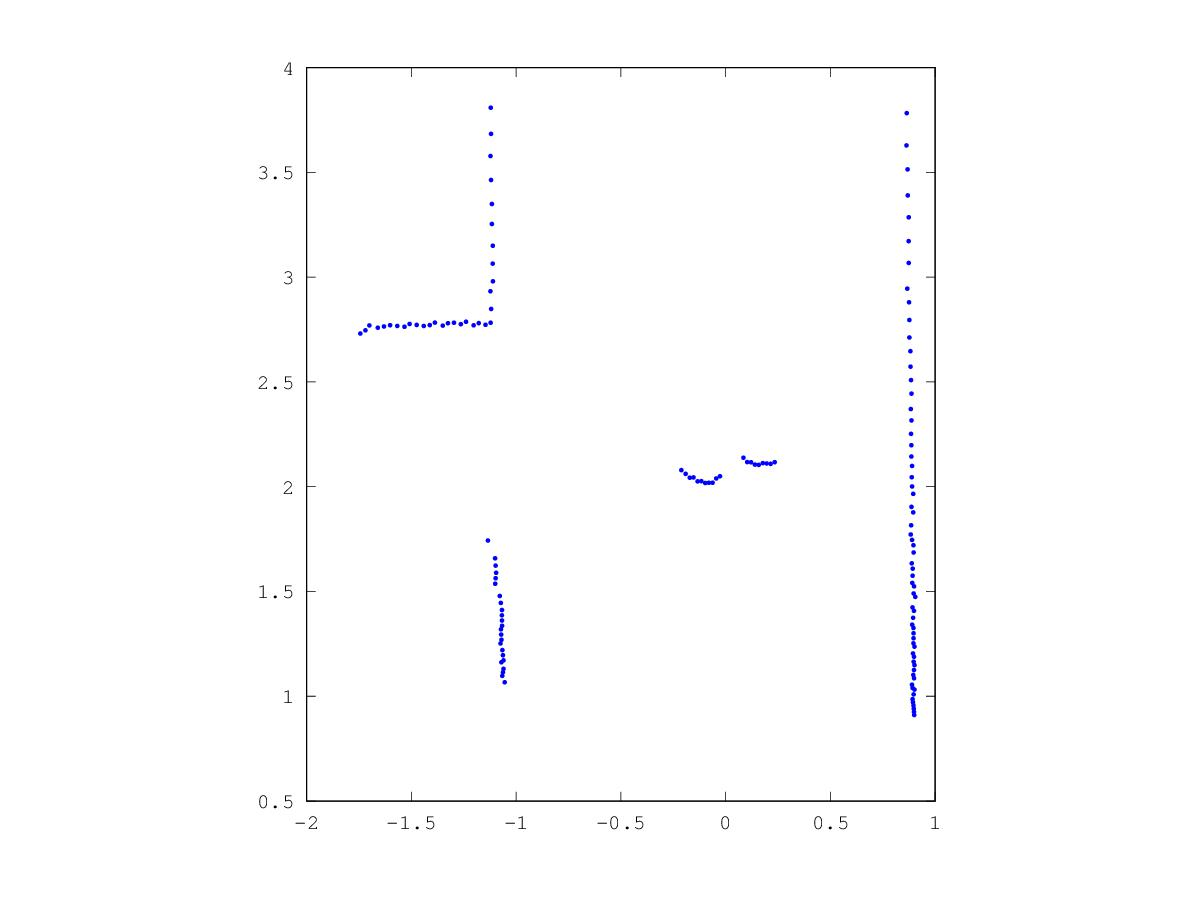
\includegraphics[width=0.5\textwidth]{presimg/human.jpg}
\caption{This plot shows a human standing in front of the robot in a hallway. The human legs are clearly visible in the center of the plot.}
\label{human}
\end{figure}

\begin{figure}
\centering
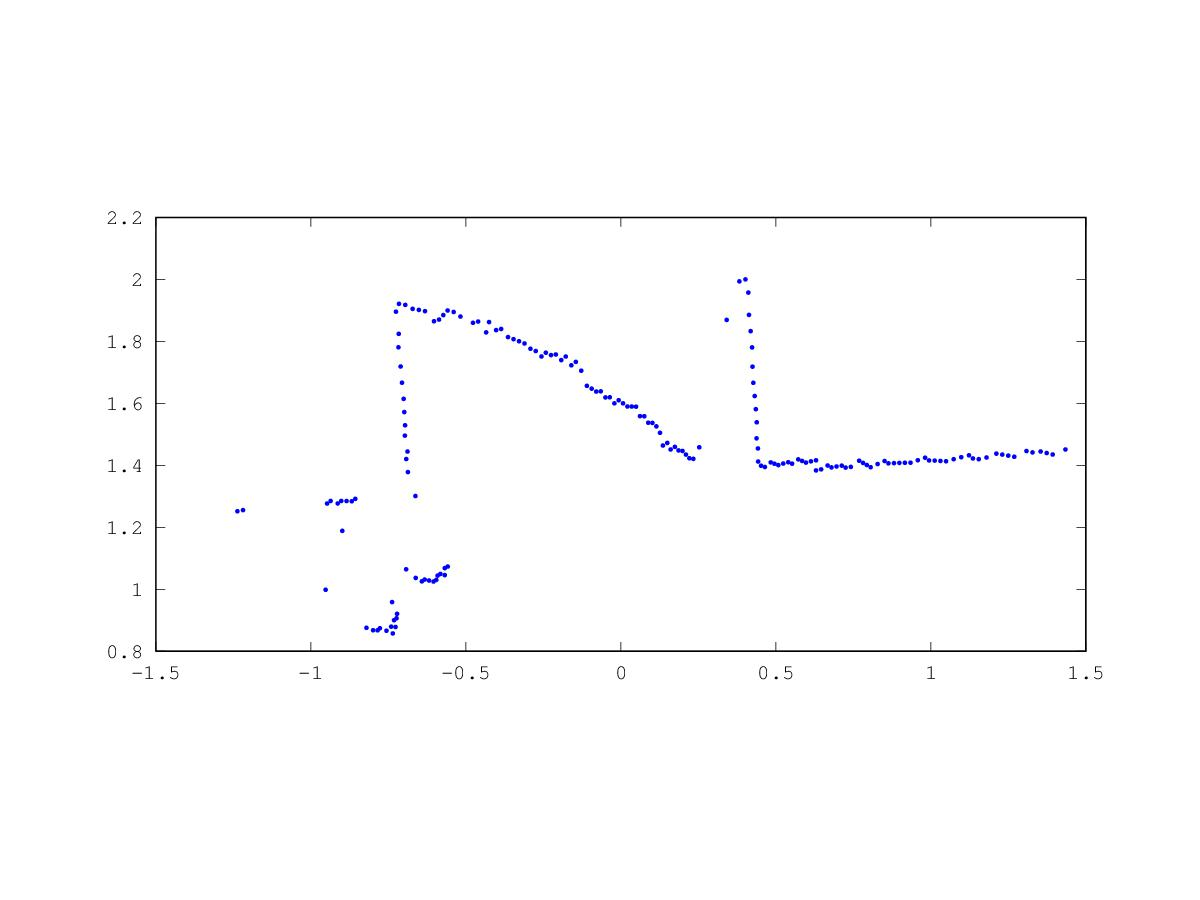
\includegraphics[width=0.5\textwidth]{presimg/doorhalf.jpg}
\caption{This plot shows a door that is half open. There is also a human standing in front of the door to the left.}
\label{doorhalf}
\end{figure}

\begin{figure}
\centering
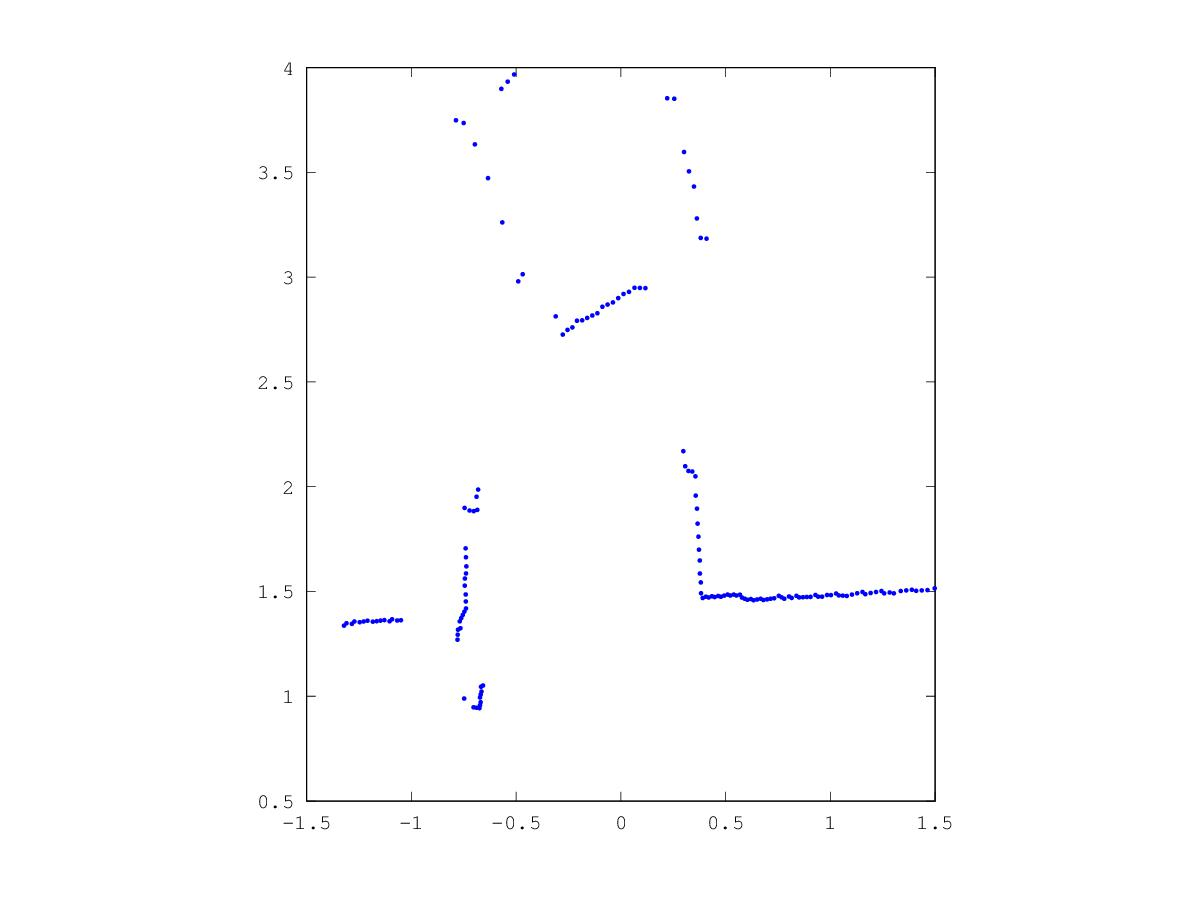
\includegraphics[width=0.5\textwidth]{presimg/doorfull.jpg}
\caption{This plots shows the same door as the plot above but now the door is fully open. Now some clutter is shown from inside the room.}
\label{doorfull}
\end{figure}

\begin{figure}
\centering
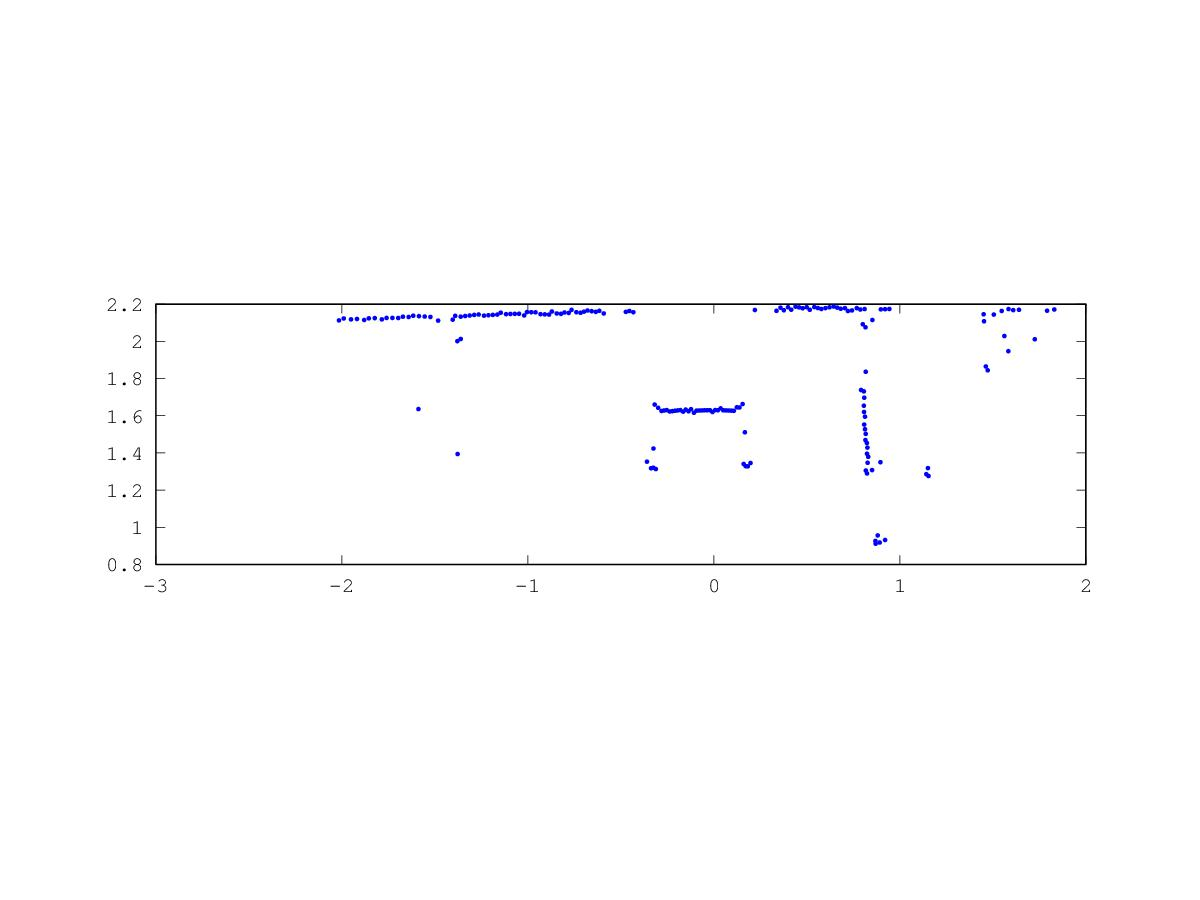
\includegraphics[width=0.5\textwidth]{presimg/chair.jpg}
\caption{This plots shows the robot standing in the middle of a room facing a wall. Right in front of the robot a chair is positioned.}
\label{chair}
\end{figure}

\section{ALGORITHM}
In this section we will explain all of the algorithms we used and how they were implemented. 

We hade two different approaches when trying to figure out a way to represent the data in a form where we could easily apply some form of machine learning on it. This was the biggest challange we had to overcome in the project. 
\subsection{Interpolation and Comparison}
After transferring the data to a form which we could more easily differentiate the characteristics of the data we decided to try a interpolation approach. This approach consisted of interpolating the data points to get a 'figure' of some sorts which we could use as a characteristic for a classifier.

The interpolation is mainly used to get an evenly distributed set of point which we could use to directly compare with another set of points to see how much error they have.

The idea behind this approach was to store measurements and their respective classifications in some sort of database. When the classifier then receives a measurement to classify the classifier would iterate over the database and using the interpolation to directly compare the new measurement with all measurements stored in the database. The classification of the best match in the database would then be assigned to the new measurement. And finally the new measurement and it's classifaction were to be stored in the database.

This idea would combine both unsupervised and supervised machine learning. The supervised learning came into play because there would need to be a databse from the start. The classifications contained in this databse had to be manually classified by us. The unsupervised learning takes place because the classifier extends it database on each run.

\subsubsection{Implementation}
We decided to start the implementation with a simple linear interpolation algorithm, that looks like:

\begin{algorithm}
  \caption{Simple lerp}\label{forward}
  \begin{algorithmic}[1]
      \State \texttt{State Probability Vector S}
      \State \texttt{Transition model T}
      \State \texttt{Observation Vector O}
      \For{\texttt{row = 0 .. S.size}}
      	\For{\texttt{col = 0 .. S.size}}
      		\State $S(row)_{next} += \alpha O(row) \cdot T(col)(row) \cdot S(col)_{prev}$
      	\EndFor
      \EndFor
  \end{algorithmic}
\end{algorithm}

\subsection{Line finding}

\subsubsection{Implementation}

\subsection{Decision Tree}

\subsubsection{Implementation}

\section{RESULTS}

\section{DISCUSSION}

\subsection{Algorithms}

\section{CONCLUSION}




%%%%%%%%%%%%%%%%%%%%%%%%%%%%%%%%%%%%%%%%%%%%%%%%%%%%%%%%%%%%%%%%%%%%%%%%%%%%%%%%



%%%%%%%%%%%%%%%%%%%%%%%%%%%%%%%%%%%%%%%%%%%%%%%%%%%%%%%%%%%%%%%%%%%%%%%%%%%%%%%%



%%%%%%%%%%%%%%%%%%%%%%%%%%%%%%%%%%%%%%%%%%%%%%%%%%%%%%%%%%%%%%%%%%%%%%%%%%%%%%%%
%\section*{APPENDIX}

%Appendixes should appear before the acknowledgment.

%\section*{ACKNOWLEDGMENT}

%The preferred spelling of the word �acknowledgment� in America is without an �e� after the �g�. Avoid the stilted expression, �One of us (R. B. G.) thanks . . .�  Instead, try �R. B. G. thanks�. Put sponsor acknowledgments in the unnumbered footnote on the first page.



%%%%%%%%%%%%%%%%%%%%%%%%%%%%%%%%%%%%%%%%%%%%%%%%%%%%%%%%%%%%%%%%%%%%%%%%%%%%%%%%

%References are important to the reader; therefore, each citation must be complete and correct. If at all possible, references should be commonly available publications.



\begin{thebibliography}{}

\bibitem{bla}blabla

\end{thebibliography}




\end{document}
